\documentclass{beamer}

\usepackage[utf8]{inputenc}
\usetheme{Pittsburgh}
\usecolortheme{crane}
\usepackage{tikz}
\usepackage{cancel}
\theoremstyle{definition}

\title{Data Representation as Low Rank Matrix Factorization}
\author{Ziv Epstein \\ \texttt{ziv.epstein@pomona.edu}}
\institute{Pomona College \\ Advised by Blake Hunter}
\date{\today}

\setbeamertemplate{navigation symbols}{}

\begin{document}
	
	\frame{\titlepage}
	%say everythng
	\begin{frame}
		\frametitle{Points in $\mathbb{R}^m$}
	\only<1>{In many contexts in data science and linear algebra,  we have lots of points in a high-dimensional space.}
		\onslide<2->{How do we cluster $x_i$? }
			\onslide<3->{ How do we perform dimensionality reduction?} %dimension of true underlying space}
				\onslide<4->{ How do we visualize them?}
			\begin{figure}
		\centering
		%introduce the dataset
			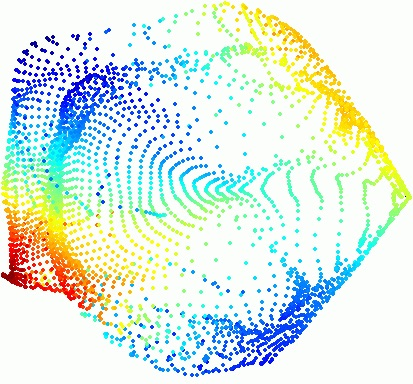
\includegraphics[width=5cm]{highD}
	\end{figure}
	\only<1>{Denote these $x_i \in \mathbb{R}^m$ for $i = 1...n$.}
	\end{frame}
	
		\begin{frame}
			\frametitle{Representation and Factorization}
		
		
		We can \textit{represent} $X \in \mathbb{R}^{n \times m}$.
				%observation v fetures
			\only<1>{\begin{figure}
				\centering
				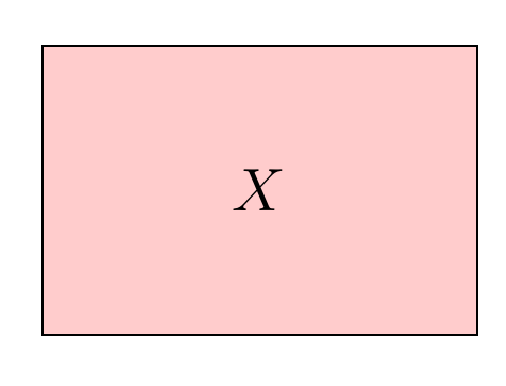
\includegraphics[height=3cm]{nnmf/nnmfA1}
			\end{figure}}
				\only<2>{\begin{figure}
						\centering
						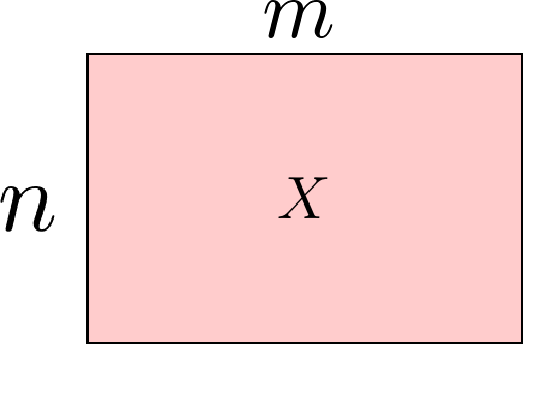
\includegraphics[height=3cm]{nnmf/nnmfA2}
					\end{figure}}
			with rank$(X) = \min(m,n)$.
		\end{frame}
		\begin{frame}
			\frametitle{Representation and Factorization} We can \textit{approximate} $X \in \mathbb{R}^{n \times m}$ as $AS$.
			\only<1>{\begin{figure}
					\centering
					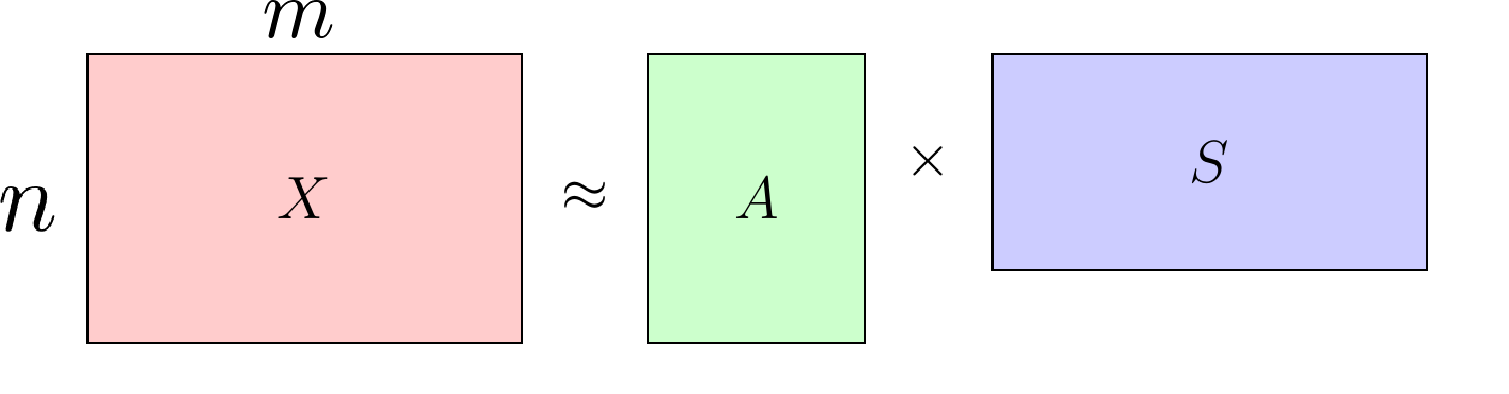
\includegraphics[height=3cm]{nnmf/nnmfA3}
				\end{figure}}
				\only<2>{\begin{figure}
						\centering
						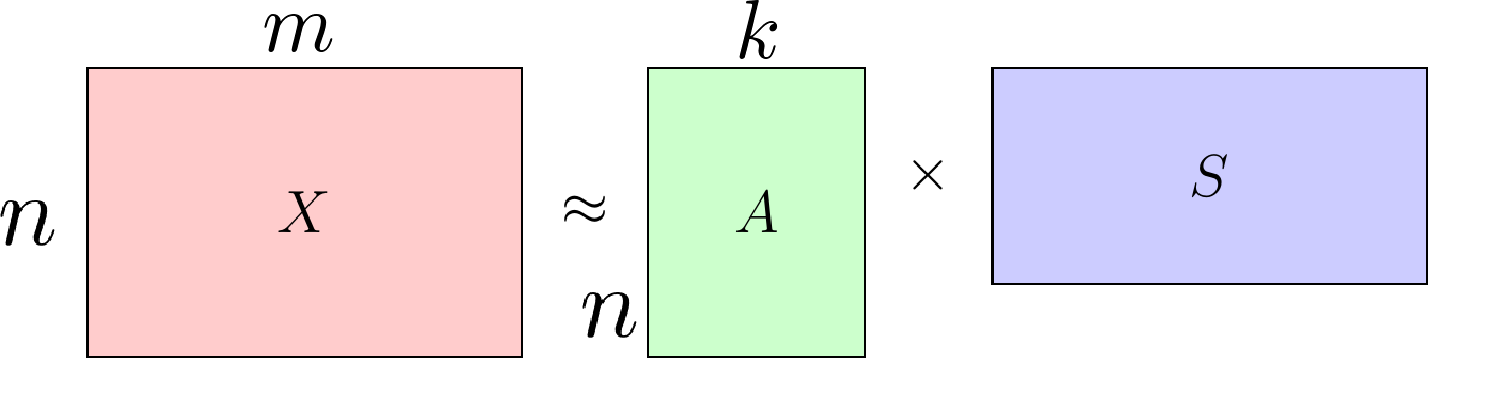
\includegraphics[height=3cm]{nnmf/nnmfA4}
					\end{figure}}
					\only<3>{\begin{figure}
							\centering
							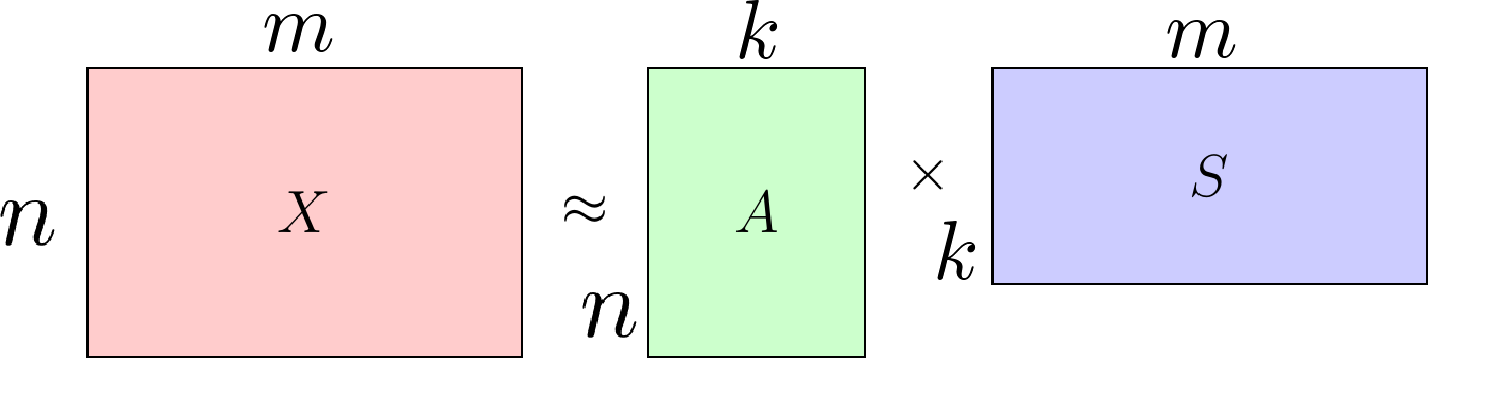
\includegraphics[height=3cm]{nnmf/nnmfA5}
						\end{figure}}
				with rank$(AS) = k << \text{rank}(X)$.
		\end{frame}
		
			\begin{frame}
				\frametitle{Low Dimensional Interpretation }
				Our original high-dimensional points are linear combinations of ``basis elements'.'
				$$x_i = \sum_{j=1 }^k A_{i,j} S_{j,\_}$$
				
		\only<2>{\begin{figure}
						\centering
						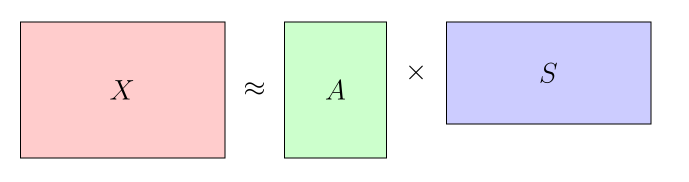
\includegraphics[height=3cm]{nnmf/nnmf1}
					\end{figure}}
					\only<3>{\begin{figure}
						\centering
						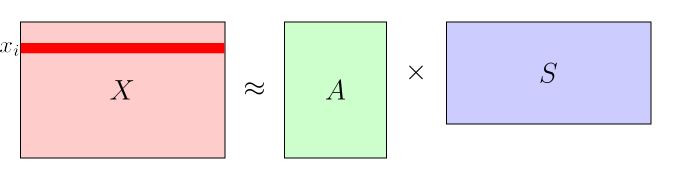
\includegraphics[height=3cm]{nnmf/nnmf2}
					\end{figure}}
					\only<4>{\begin{figure}
							\centering
							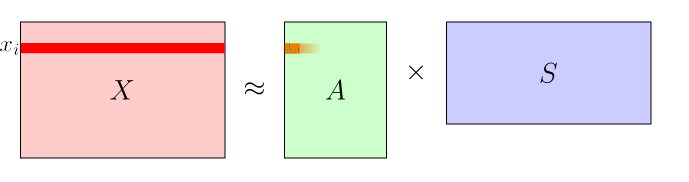
\includegraphics[height=3cm]{nnmf/nnmf3}
						\end{figure}}
							\only<5>{\begin{figure}
									\centering
									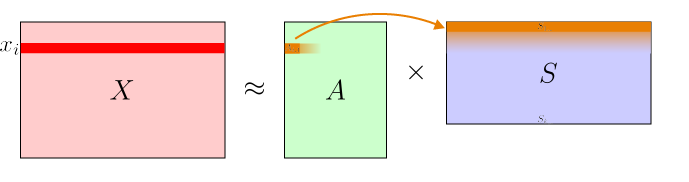
\includegraphics[height=3cm]{nnmf/nnmf4}
								\end{figure}}
									\only<6>{\begin{figure}
											\centering
											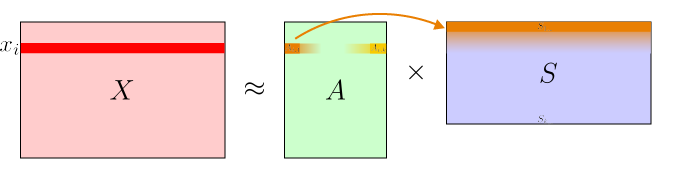
\includegraphics[height=3cm]{nnmf/nnmf5}
										\end{figure}}
											\onslide<7-8>{\begin{figure}
													\centering
													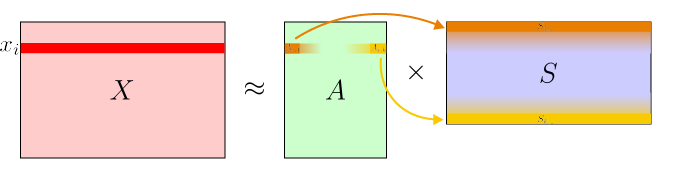
\includegraphics[height=3cm]{nnmf/nnmf6}
												\end{figure}}
					\onslide<8>{Find factorization by solving optimization problem $$\min_{A,S} ||X-AS||$$}.
			\end{frame}
			
			\begin{frame}
						\frametitle{Example (Lee and Seung 1999)}
					\onslide+<2->{
					A 19x19 pixel greyscale image of a face is a data point ($x_i \in \mathbb{R}^{361}$ with values between 0 and 256)}
				\only<2>{	\begin{figure}
						\centering
						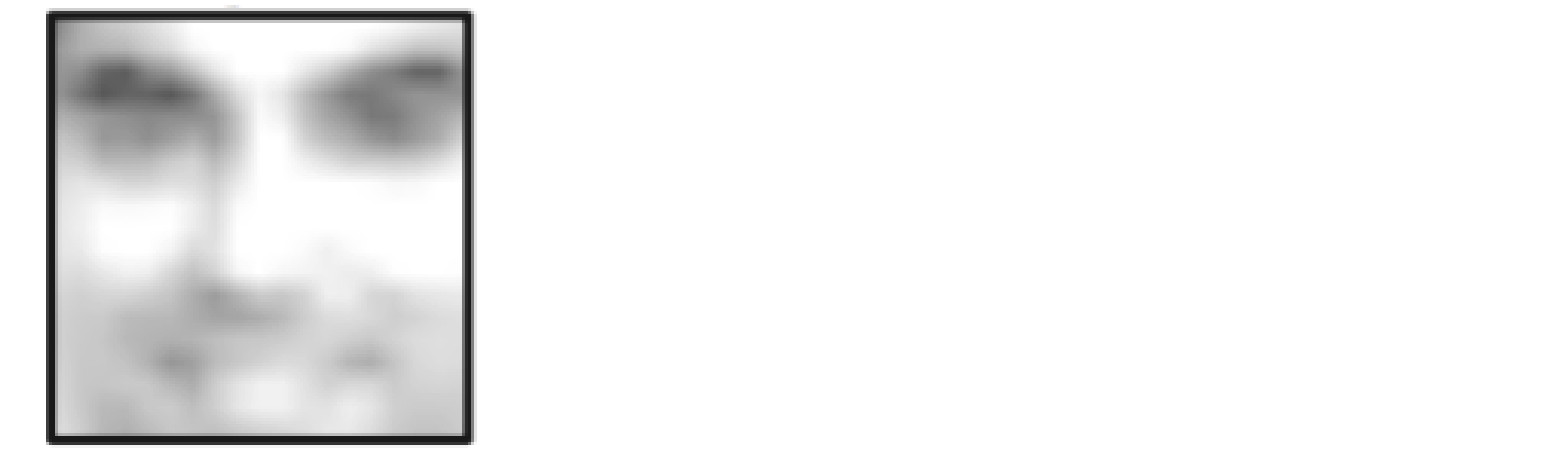
\includegraphics[height=3cm]{face/face1}
					\end{figure} }
						\only<3-4>{	\begin{figure}
								\centering
								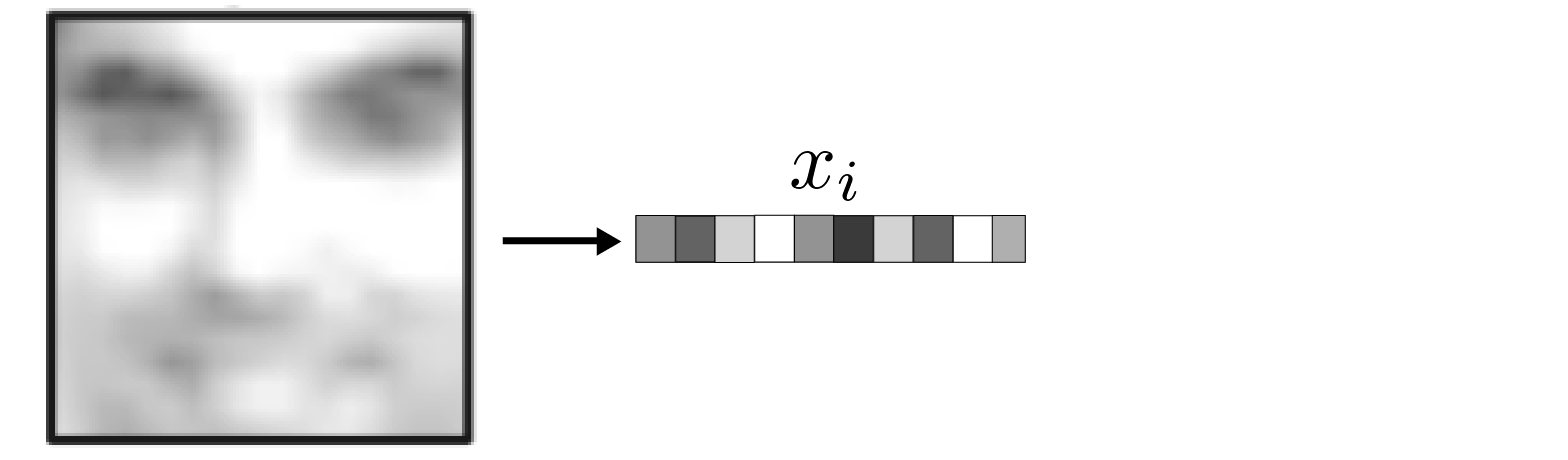
\includegraphics[height=3cm]{face/face2}
							\end{figure} }
								\only<5>{	\begin{figure}
										\centering
										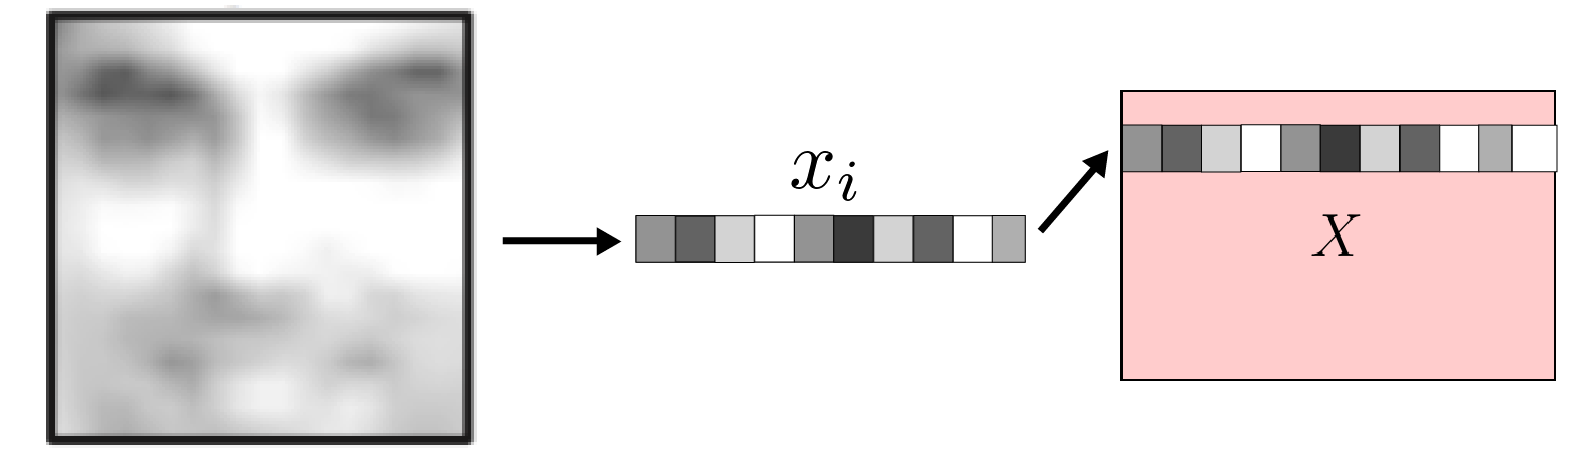
\includegraphics[height=3cm]{face/face4}
									\end{figure} }
									\onslide+<4->{Take a database of 2,429 faces to get $X \in \mathbb{R}^{2429 \times 361}$}
					\end{frame}
					
							\begin{frame}
								\frametitle{Example (Lee and Seung 1999)}
							\onslide<1->{\textbf{Before:} Find $A$ and $S$ such that $||X-AS||$ is minimized.
								\begin{figure}
									\centering
									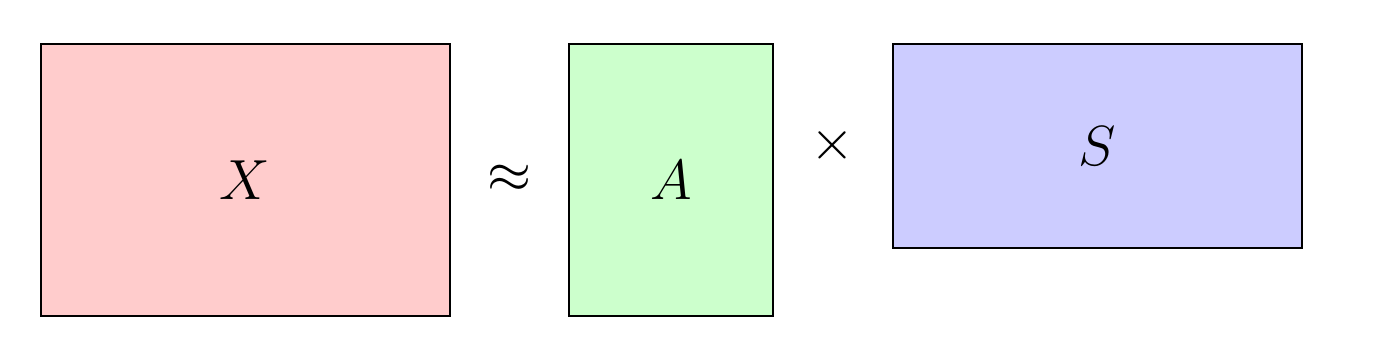
\includegraphics[height=2cm]{nnmf}
								\end{figure}}
								\onslide<2->{\textbf{Now:} We add some constraints 
									\begin{enumerate}
										\onslide<3->{\item Columns of $A$ to be orthonormal; Rows of $S$ to be orthogonal (PCA)}
										\onslide<4->{\item All entries of $A$ and $S$ are non-negative (NMF)}
										%X is non-negative distribution over pixels, force A and s to be distrubtions as well
									\end{enumerate}}
										\onslide<5->{For each, find $A$ and $S$ subject to constraints that minimize 
											$$||X-AS||$$}
								\end{frame}
									\begin{frame}
										\frametitle{Example (Lee and Seung 1999)}
											\onslide<1->{\begin{figure}
													\centering 1: PCA
													\onslide<2->{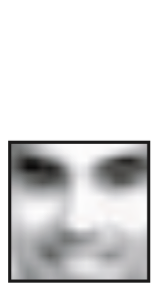
\includegraphics[height=2.4cm]{face-imp/pcaFACE2}
\includegraphics[height=2.4cm]{face-imp/eq}}
													\onslide<3->{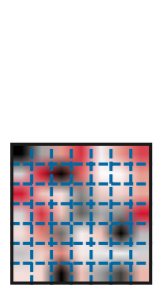
\includegraphics[height=2.4cm]{face-imp/pcaFACE1}}
													\onslide<4->{
\includegraphics[height=2.4cm]{face-imp/x}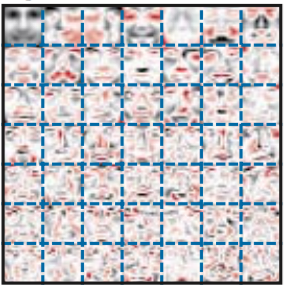
\includegraphics[height=2.4cm]{face-imp/pcaFACE}}
													\onslide<5->{``eigenfaces''}
													%weights
												\end{figure}}
				
										
												\onslide<6->{\begin{figure}
														\centering 1: NMF
														\onslide<7->{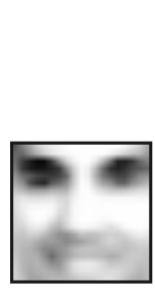
\includegraphics[height=2.4cm]{face-imp/nmfFACE2}
\includegraphics[height=2.4cm]{face-imp/eq}}
														\onslide<8->{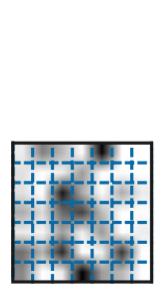
\includegraphics[height=2.4cm]{face-imp/nmfFACE1}}
														\onslide<9->{
\includegraphics[height=2.4cm]{face-imp/x}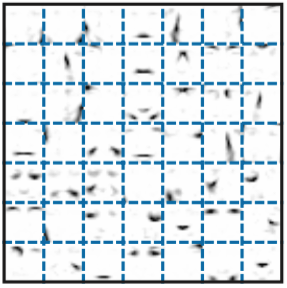
\includegraphics[height=2.4cm]{face-imp/nmfFACE}}
														\onslide<10->{parts based}
														%weights
													\end{figure}}
										\end{frame}
		\begin{frame}
			\frametitle{Recognition-by-parts}
			NMF learns an additive, parts based model
				\only<1>{\begin{figure}
				\centering
			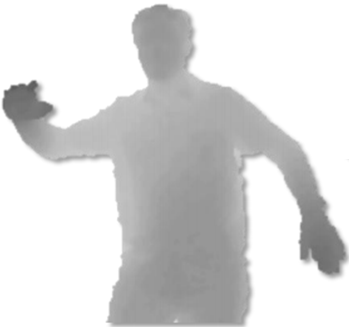
\includegraphics[height=2.4cm]{dingusBefore}
					\end{figure}}
			
				\only<2>{\begin{figure}
						\centering
						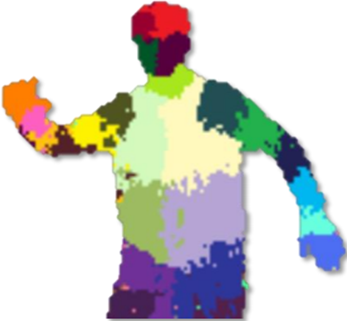
\includegraphics[height=2.4cm]{dingus}
						\end{figure}
							which is what our brain does when recognizing images!}
					
			
			\end{frame}
			
				\begin{frame}
					\frametitle{Recognition-by-parts}
					There is a lot of evidence in cognitive science that we understand high level concepts using a parts-based representation
					\onslide<2-4>{\begin{enumerate}
						\onslide<2-4>{\item Minsky, Marvin. "A framework for representing knowledge." (1974)}.
						\onslide<3-4>{\item Palmer, Stephen E. "Hierarchical structure in perceptual representation." Cognitive psychology 9.4 (1977): 441-474.}
							\onslide<4>{\item Biederman, Irving. "Recognition-by-components: a theory of human image understanding." Psychological review 94.2 (1987): 115.}
					\end{enumerate}}
				\end{frame}
				\begin{frame}
						\frametitle{Recognition-by-parts}
						\only<1>{	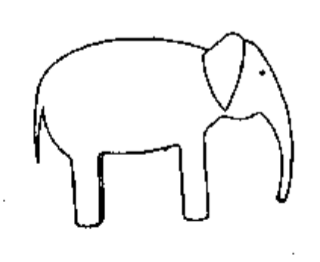
\includegraphics[height=2cm]{el1}}
						\only<2-4>{	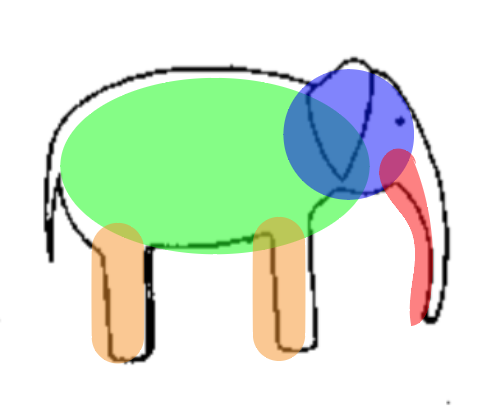
\includegraphics[height=2cm]{el2}}
						\only<3-4>{	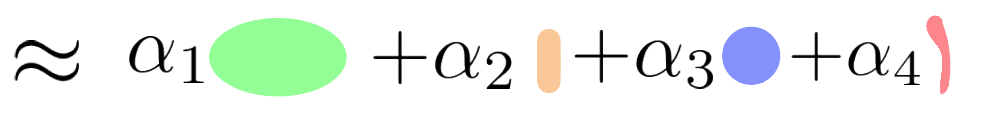
\includegraphics[height=1cm]{el3}}
						\onslide<4>{	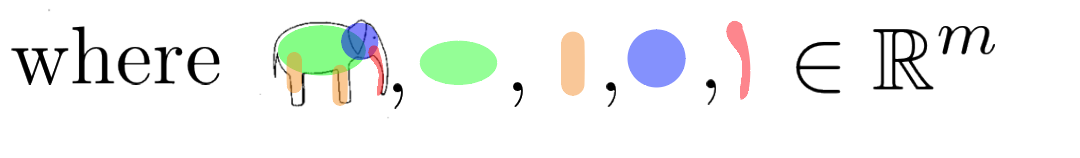
\includegraphics[height=1.5cm]{el4}}
						
					\end{frame}
					
							\begin{frame}
								%easily generalized to text
								%connection between sludes (S is the topic representations over words)
								\frametitle{Topic Modelling}						
									\only<2-4>{	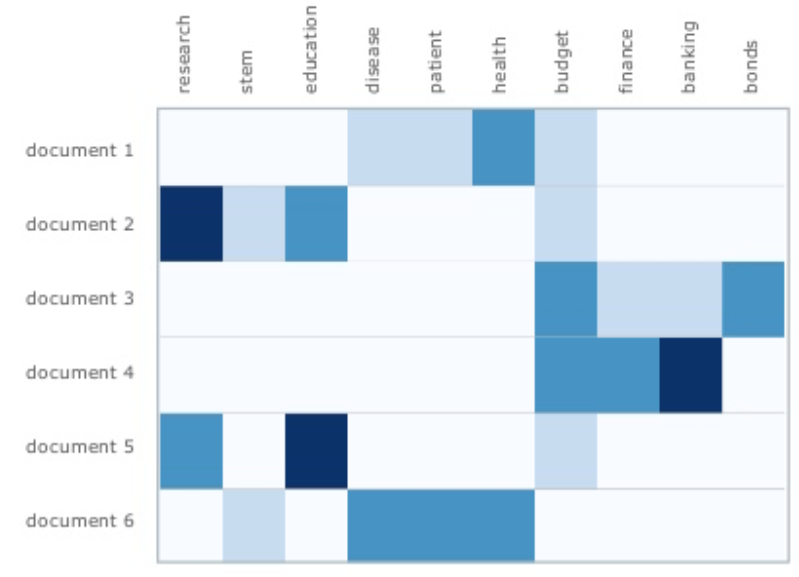
\includegraphics[height=4cm]{tmodX}}
									\only<3-4>{	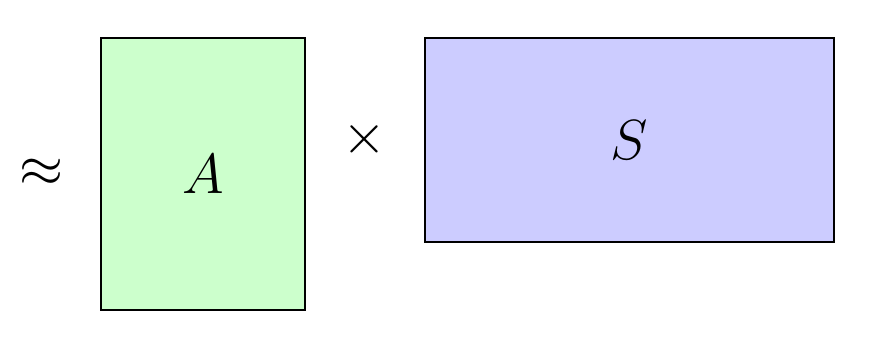
\includegraphics[height=1.8cm]{tmodF}}
									\onslide<4>{	Perform with corpus of news documents with $k=10$}
								\end{frame}
								\begin{frame}
										\frametitle{Topic Modelling}			
									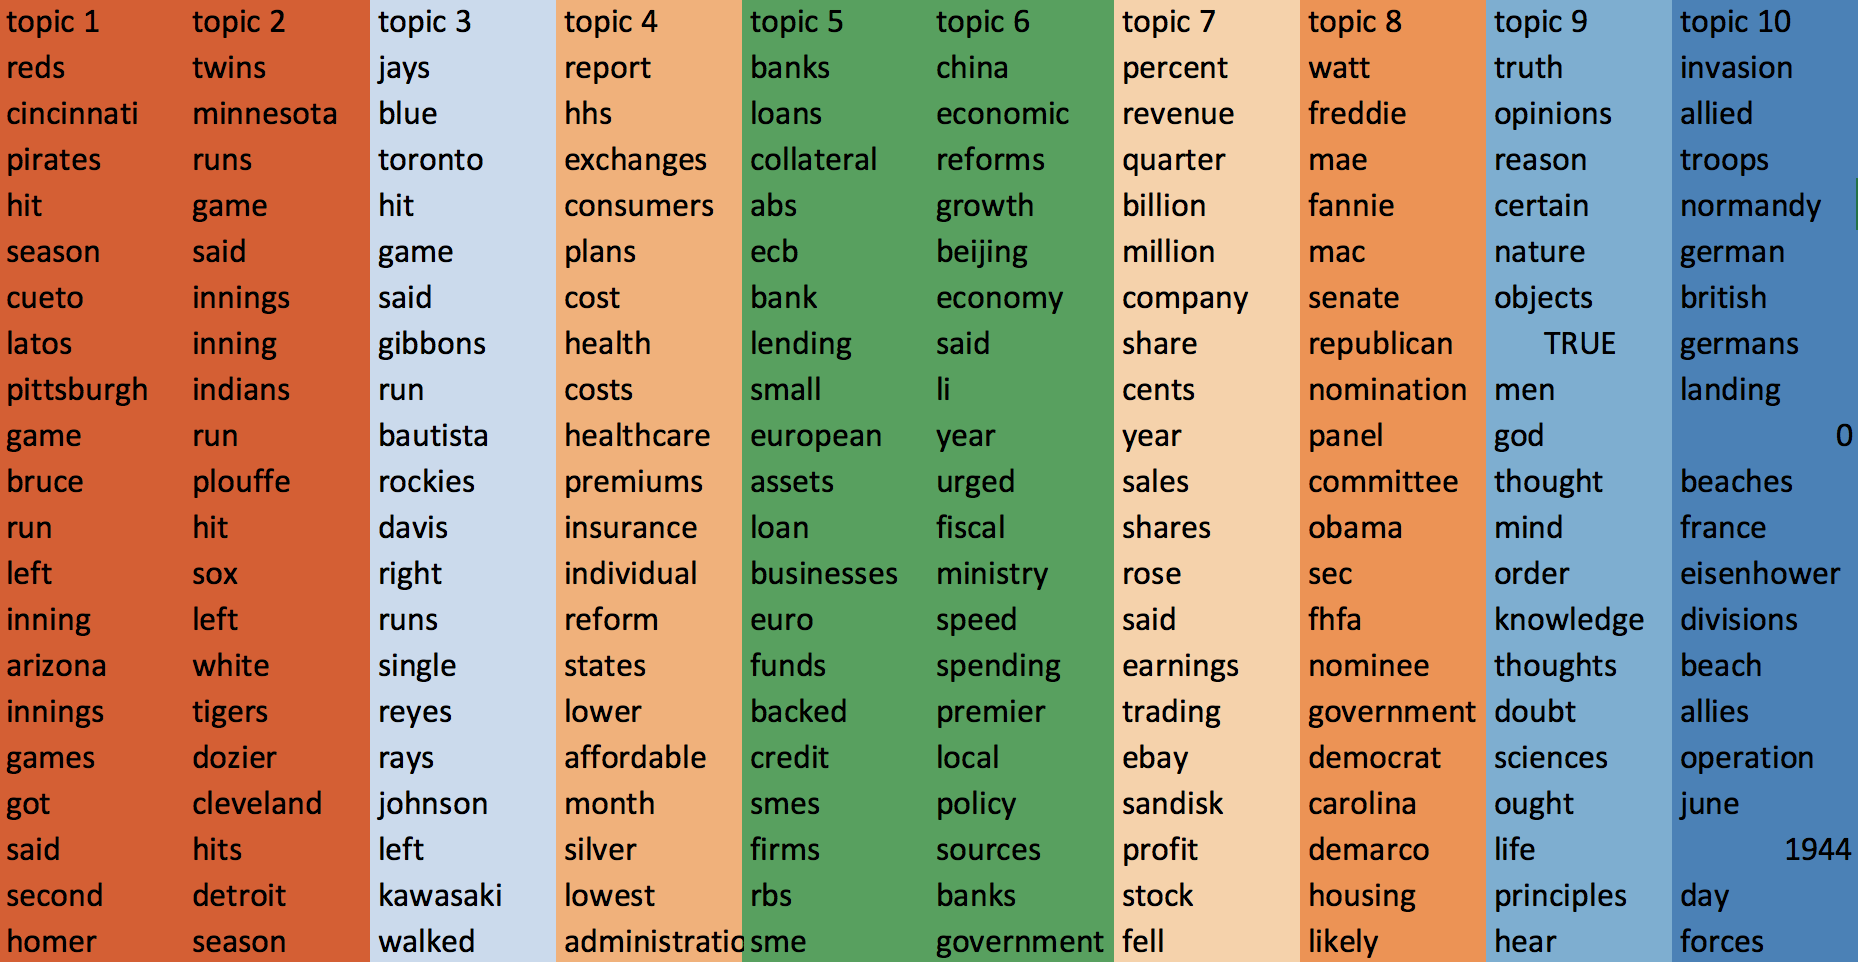
\includegraphics[height=5.5cm]{topic}
							
								\end{frame}
								\begin{frame}
										\frametitle{One final application}
							
								\begin{columns}
									\onslide<2-4>{\begin{column}{0.48\textwidth}
										Graph clustering! 
											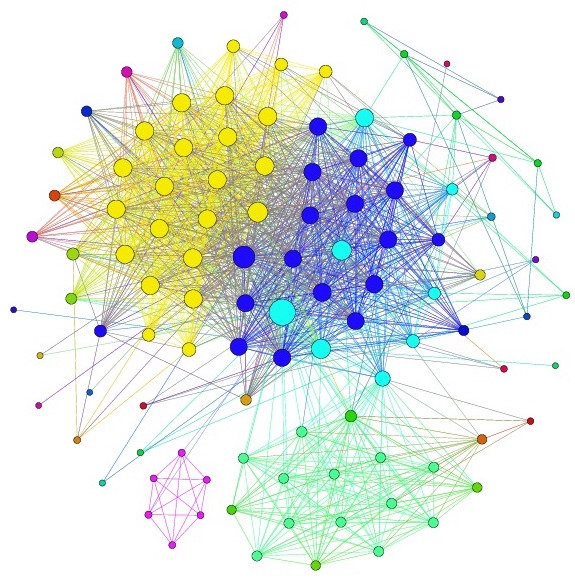
\includegraphics[height=5cm]{cluster}
									\end{column}}
									\onslide<3-4>{\begin{column}{0.48\textwidth}
										\begin{definition}
											A  \alert{clustering} $C = \{C_1,  \cdots , C_k\}$ of a graph $G=(E,V)$ is a partition of the vertices. A \alert{good clustering} optimizes some measure of community.
										\end{definition}	}
										
									\end{column}
								\end{columns}
								
								\onslide<4>{$$\text{connectivity}(G,C) = \frac{\#\{(i,j)\in E | (i,j) \in C\} + \#\{(i,j)\not\in E | (i,j) \not\in C\}}{|V|^2}$$}
									
												
								\end{frame}
								\begin{frame}
									%edges within group and complement
									\frametitle{Graph Clustering}
					\onslide<1->{The clustering $C$ can be formulated as a membership matrix $M \in \{0,1\}^{n \times k}$ with $M_{ir}=1$ if $i \in C_r$ and $M_{ir}$ if $i \not\in C_r$. }
					\begin{align*}\onslide<2->{\text{connectivity}(G,C)  &= 1-\frac{\sum_{i,j} \left(X_{ij} - \sum_{r=1}^k M_{ir}M_{jr}\right)^2}{|V|^2}\\}
					\onslide<3->{&=1-\frac{||X-MM^T||^2_F}{|V|^2}}
					\end{align*}
					\onslide<4->{Finding a clustering $C$ that maximizes the connectivity is equivalent to the minimization problem}
					\only<4>{$$\min_{M \in \{0,1\}^{n\times k}} ||X-MM^T||^2_F$$}
						\onslide<5->{$$\cancel{\min_{M \in \{0,1\}^{n\times k}} ||X-MM^T||^2_F}$$}
					\onslide<6->{$$\min_{M \in \mathbb{R}_{+}^{n\times k}} ||X-MM^T||^2_F$$}
					\onslide<7->{where $M$ is a \alert{weak membership matrix}. That is, the larger $M_{i,j}$, the stronger membership of vertex $i$ in cluster $j$. }		
						\end{frame}	
							\begin{frame}
								\frametitle{Conclusion}
								\begin{itemize}
									\onslide<2->{\item 	Many important problems are actually NMF in disguise!}
										\onslide<3->{\item 	Powerful, visual and intuitive technique for any data set that can be represented as a matrix}
										\onslide<4->{\item My thesis also explores:}
									
									\begin{itemize}
											\onslide<5->{\item more types of NMF and relation to cognition: supervised, hierarchical}
										\onslide<6->{	\item neural networks, they can even be thought of as recursive NMF!}
											\onslide<7->{	\item  Visualization techniques and implementations}
									\end{itemize}
								\end{itemize}
								\begin{figure}
									\centering
										
\includegraphics[height=4.5cm]{conc}
								\end{figure}
								
								\end{frame}	
								\begin{frame}
										\begin{figure}
											\centering
											
\includegraphics[height=4.5cm]{thanks}
										\end{figure}
										\begin{figure}
											\centering
											
\includegraphics[height=4.5cm]{conc}
										\end{figure}
								\end{frame}
						
\end{document}